\chapter{Investigating the sub-continental ancestry of ethnic minorities within the UK Biobank from sparse genotype data}
\label{chapterlabel3}

\section{Introduction}

From a genetic standpoint, the British population is one of the most studied in the world, with many different studies sequencing or genotyping individuals from across the U.K (e.g. \cite{bycroft2018uk, Leslie2015, turnbull2018introducing, uk10k2015uk10k}). These studies have been primarily aimed at researching the genetic basis of disease, but have also been used to investigate population history, substructure  and the relationship of different sub-populations in the U.K. to other European countries \cite{Leslie2015, schiffels2016iron, liu2020human}.  

The U.K. is also an ethnically diverse country, with 13.8\% of individuals belonging to ethnic minority groups (source: \href{https://www.ons.gov.uk/peoplepopulationandcommunity/populationandmigration/populationestimates/articles/researchreportonpopulationestimatesbyethnicgroupandreligion/2019-12-04}{ONS survey}). Groups of people from across the world have migrated to the U.K. at different periods in the previous 3 centuries, driven by the legacy of colonialism, the transatlantic Slave Trade and economic reasons. Despite this, the roughly 9 million ethnic minorities within the U.K. remain relatively understudied in the context of genetics. For example, every one of the 27 papers in the GWAS catalog with "UK Biobank" in the title, and 2 others presently in the catalog curation queue, limited their analyses to subgroups described in various terms as "White British", "British" "European" "White European" "Caucasian" or "White" \cite{manolio2019using}. The primary reason for this is reasonable concerns over the confounding effect of population substructure within a cohort \cite{hellwege2017population}; retaining a more genetically homogeneous cohort is one strategy to mitigate this. 

Evidence is mounting that the results from GWAS, including Polygenic Risk Scores (PRS), may not be transferrable to other populations if they have been conducted in cohorts of exclusively European individuals \cite{kuchenbaecker2019transferability, martin2017human, bustamante2011genomics}. The reasons for this is currently unclear, but it has been suggested that differences in LD structure may be the cause \cite{vilhjalmsson2015modeling}. Ethnic minorities may therefore miss out on the advances in healthcare driven by large-scale genomic projects. Understanding the population structure of ethnic minorities within the U.K. Biobank is an important step towards including a diversity of ancestries in GWAS [not totally sure if this is true]. 

During my PhD, I obtained the `Human Origins' dataset which, at the time of writing, is the most detailed dataset of genotype data from African individuals. Whilst the dataset contains individuals from across Africa, it contains particularly large numbers of individuals from South Africa (n=104), Cameroon (n=567) and Ghana (n=211), which are countries known to have contributed immigrants to the U.K. Therefore, this dataset is ideal for use as a reference panel to investigate the ancestry of ethnic minorities within the U.K. Biobank. In particular, I am interested in investigating the ancestry of individuals with recent African ancestry. 

One potential issue is that only 70,776 SNPs overlap between the U.K. Biobank and Human Origins genotyping arrays. This is much lower than the number used in a typical ChromoPainter analysis, which is usually betweeen 500,000 and 700,000. Using a low number of SNPs in the analysis may reduce the power to infer accurate ancestry proportions, as there is less data points to compare populations with. Therefore, one option is to impute the non-overlapping SNPs using a reference panel. However, the effect of imputation on ChromoPainter-style analyses has yet to be fully investigated. It is possible that imputing a large number of positions may introduce biases, particularly towards populations which are present in the reference panel. Studies have shown repeatedly that genotypes in non-European individuals are imputed less accurately compared to European individuals. Accordingly, we can ask whether it is preferable to retain a smaller number of non-imputed SNPs or a larger number of imputed SNPs. I will investigate this in this chapter. 

This chapter will focus on two questions. Firstly, I am interested in relating the genetic variation of individuals in the U.K. Biobank with recent African ancestry to the populations in the Human Origins dataset. 


\section{Methods}

\subsection{U.K. Biobank data access and initial processing}

Access was obtained to study the U.K. Biobank dataset via UCL Genetics Institute. 

I first downloaded the U.K. Biobank genotype data, consisting of 488,377 individuals genotyped at 784,256 genome-wide SNPs on the UK Biobank Axiom Array. I will hereafter refer to this data as the `non-imputed' data. plink1.9 \cite{purcell2007plink} was used to convert the binary plink files to \texttt{.bcf} format. I identified strand inconsistencies between the UK Biobank and Human Origins using the gt-conform utilty from Beagle (\url{https://faculty.washington.edu/browning/conform-gt.html}) and removed any inconsistent positions. 

I also download U.K. Biobank data which had already been imputed to approximately 96m SNPs. Data was imputed using the combined references of the Haplotype Reference Consortium (HRC) and UK10K haplotype resource. Full details of imputation can be found in the paper of McCarthy et al (2016) \cite{mccarthy2016reference}. The imputed data was downloaded and converted from \texttt{.bgen} to \texttt{.bcf} format using qctool2 (\url{https://www.well.ox.ac.uk/~gav/qctool_v2/}). Strand inconsistencies between the UK Biobank imputed dataset and Human Origins dataset were identified using the gt-conform utilty from Beagle and any inconsistent positions removed.

\subsection{Data preparation - Human Origins}

To determine the ancestry patterns in U.K. Biobank individuals, it is necessary to compare them to reference dataset of individuals of known origin. As I am particularly interested in studying individuals with recent African ancestry, the Human Origins dataset (appendix A.20) is ideal for this purpose, as it contains many individuals from many different ethnic groups from across Africa (Fig. \ref{HumanOriginsMap}) 

\begin{sidewaysfigure}[htp]
    \centering
    \includegraphics[width=1.0\textwidth]{../images/chapter3/HumanOriginsMap.pdf}
    \caption{adfdsfsdg.}
    \label{fig:HumanOriginsMap}
\end{sidewaysfigure}

\subsection{ADMIXTURE analysis}

Performing chromopainter analysis on the entire UK Biobank dataset (n=488,377 individuals) is currently computationally infeasible. Thus, I chose to analyse only those individuals with more than 50\% non-European ancestry. ADMIXTURE is a fast and accurate way to estimate continental-scale ancestry proportions.

I first LD pruned the non-imputed U.K. Biobank dataset using using the \texttt{plink --indep-pairwise 50 10 0.02} \cite{purcell2007plink}. This left a total of  70,776 bi allelic SNPs. I then subsetted the 1000 genomes dataset down to the 70,776 SNPs retained in the U.K. Biobank dataset and merged them using \texttt{bcftools merge}. Thus, I had a dataset containing all U.K. Biobank and 1000 genomes individuals, genotyped at 70,776 SNPs.

I ran a supervised ADMIXTURE analysis on each batch by using the \texttt{--supervised} command and fixing the 4 reference populations as GBR British, Nigeria Yoruba, Han Chinese and Gujarati Indian. The rest of the arguments were left to default.

\subsection{Data preparation - non imputed data}

It is necessary to merge datasets in order to jointly analyse them with ChromoPainter. I therefore merged the Human Origins and non-imputed U.K. Biobank datasets. I first identified which SNPs were common to both datasets and then subsetted both so that they contained only those SNPs, resulting in a total of 65,749 SNPs. I then merged the two datasets using \texttt{bcftools merge}. I only retained U.K. Biobank individuals if they had 50\% non-European ancestry or more, resulting in a total of 26,298 individuals. 

I phased the merged UK Biobank / Human Origins dataset using shapeit4 \cite{delaneau2018integrative}. I set \texttt{--pbwt-depth 8} and left all other parameters as default. The resulting \texttt{.bcf} of phased haplotypes was converted to chromopainter format using a custom script \url{https://github.com/sahwa/vcf_to_chromopainter}.  

\subsection{Data preparation - imputed data}

Similarly to above, I needed to merge the imputed Biobank data with the Human Origins dataset. Again, I filtered both datasets to retain only SNPs which were common to both the datasets. The Human Origins and UK Biobank datsets were then merged using the \texttt{bcftools merge} command. The resulting merged dataset contained 493,407 individuals and 535,544 SNPs.

The merged dataset was then phased using shapeit4 \cite{delaneau2018integrative}, setting \texttt{--pbwt-depth 1} to increase speed at this large sample size. The phased output was converted to chromopainter output using a custom script (\url{https://github.com/sahwa/vcf_to_chromopainter}).

\subsection{Imputation bias test}

Imputing variants in non-European individuals using a reference panel that is primarily composed of European individuals may lead to biased or inaccurate imputation. To explicitly evaluate this possibility, I performed a test of the effect of imputation using the Human Origins dataset as a `truthset'.
 
I took the full Human Origins dataset (5998 individuals and 560,420 SNPs) and submitted it to the Sanger Imputation Server \url{https://imputation.sanger.ac.uk/}, using the full Haplotype Reference Consortium (HRC) as a reference for phasing and imputation. This reference panel was chosen because it was the same one used for imputing the U.K. Biobank individuals.

I next subsetted the imputed Human Origins dataset down to SNPs present in the UK Biobank array, leaving 727,325 positions present in the imputed Human Origins dataset. I then performed an `all-v-all' painting, forming each target haplotype as a mosaic of all other haplotypes. I also performed an identical `all-v-all' painting of the same Human Origins dataset, but using the original set of SNPs where none had been imputed. 

Therefore, I had 2 co-ancestry matrices of identical structure, but one was generated using imputed SNPs and the other was generated using no imputed SNPs. 

I also performed SOURCEFIND analysis on both matrices. Individuals were grouped into populations and all populations were used as surrogates for each target population. Default parameters were used and each SOURCEFIND target was analysed for 2,000,000 MCMC iterations. Ancestry proportions and confidence intervals were estimated from the raw MCMC output using the Coda R library \cite{oro22547}.

\subsection{Chromopainter}

I performed 2 identical paintings using the imputed and non-imputed datasets. Both used all Human Origins samples as donors and all U.K. Biobank individuals with more than 50\% non-European ancestry as recipients. This allowed me to characterise the latent ancestry of each of the selected U.K. Biobank individuals in terms of known Human Origins populations. Each autosome was painted separately and the resulting files merged using chromocombine-0.0.4 (\url{https://people.maths.bris.ac.uk/~madjl/finestructure-old/chromocombine.html}).

For SOURCEFIND analysis, a surrogate must be painted by the same set of donor groups as the target individuals. Therefore, I also performed an `all-v-all' painting of the Human Origins dataset(see below section) and combined this coancestry matrix with that obtained from painting each Biobank individual with the Human Origins.

\subsection{SOURCEFIND}

I wanted to estimate ancestry proportions for each of the selected U.K. Biobank individuals using SOURCEFINDv2 \cite{Chacon-Duque2018}. I used the combined painting from the section above. I analysed each U.K. Biobank individual in turn, using all Human Origins populations as surrogates.

\section{Results}

\subsection{4\% of UK Biobank individuals have at least 50\% non-European ancestry}

As performing ChromoPainter analysis on the approximately 500,000 individuals would be computationally unfeasible, I performed supervised ADMIXTURE on all 488,378 UK Biobank individuals in order to identify individuals with at least 50\% non-European ancestry. These individuals would then be carried forward to later ChromoPainter analyses. In total, there were 8476, 2653, 9171 individuals with at least 50\% ancestry from Yoruba, Han Chinese and Gujarati reference populations respectively, corresponding to 4.16\% of the total U.K. Biobank individuals. Although I use these labels, it is important to note that an individual with e.g. 50\% `Han Chinese' ancestry does not necessarily derive 50\% of their ancestry from the Han Chinese population, but that 50\% of their ancestry most closely matches Han China relative to the other reference populations. Thus, a Japanese individual may be modeled as 100\% Han Chinese whilst not being Han Chinese in an ethnic sense. Similarly, for brevity, I will refer to individuals who have more than 50\% of their ancestry from Yoruba as being `African' Biobank individuals, whilst acknowledging `African' as a broad label which encompasses a large diversity of ancestries and ethnicities.  

I chose to validate the ADMIXTURE results to ensure that there has not been any mixing of individual labels or that ADMIXTURE has been run for an adequate number of iterations. To do this, I selected all individuals who self-identified as being either "Caribbean", "African" or "Black or Black British" (n=7527) and assessed the distribution of ADMIXTURE ancestry proportions, under the assumption that these individuals should contain more African than other kinds of ancestry. This was the case, with the mean proportion of African ancestry among these individuals being 0.85 (Fig. \ref{fig:African_Inds_proportions_ADMIXTURE}).

However, there was substantial variation in the ancestry proportions for those self-identified as being either "Caribbean", "African" or "Black or Black British" - proportions of Yoruban and British ancestry ranged from 0.00001 to 1, Han Chinese from 0.00001 to 0.53 and Gujarati from 0.759 to 0.00001, reflecting the diverse array of genetic ancestries that can fall under a given ethnic label. Indeed, this is evidence that relying on self-reported ethnicity may yield variable results when e.g. used as a covariate in a GWAS. For example, there were 48 people who self identified as being either "Caribbean", "African" or "Black or Black British", but had less than 1\% African ancestry.

\begin{figure}[htp]
    \centering
    \includegraphics[width=1.0\textwidth]{../images/chapter3/African_Inds_proportions.pdf}
    \caption{Ancestry proportions inferred from supervised Admixture run (k=4) for all individuals who self identified as being either "Caribbean", "African" or "Black or Black British"}
    \label{fig:African_Inds_proportions_ADMIXTURE}
\end{figure}

\subsection{To impute or not?}

In order to utilise the Human Origins dataset, it is necessary to merge it with the UK Biobank dataset. It is only possible to retain SNPs that have been genotyped in both datasets when merging datasets for ChromoPainter analysis. The overlap between the two datastets was 70,776 SNPS, an order of magnitude fewer than in a typical ChromoPainter analysis. Using fewer SNPs risks losing power to detect fine-scale differences between populations, so one option is to boost the number of SNPs using imputation. The imputed dataset consisted of 535,544 SNPs in total, 87.7\% of which were imputed. However, having a high percentage of imputed SNPs may bias downstream analyses. Therefore, it is important to determine whether it is preferable to use fewer imputed SNPs or a larger number of imputed SNPs.

I performed two related tests to determine whether using a sparse set of approximately 70,000 non-imputed SNPs or approximately 70,000 non-imputed and 430,000 imputed SNPs generates a more accurate painting. I selected a set of ethnic groups from Nigeria, Cameroon and Ghana and painted them using a fixed set of donors. I randomly assigned half of the individuals from each ethnic group to be `donors' and half to be `recipients' and painted each group of recipients using all other `donors'. One way to test the reliability of a painting is by testing whether individuals copy more from other individuals in their own populations than individuals from other populations. For both the imputed and non-imputed datasets, I calculated pairwise $TVD$ between all individuals and then aggregated the values by population. $TVD$ is a distance metric which is the sum of the absolute differences between two copyvectors. When using the imputed data, 30\% of the recipient populations had the lowest TVD with their own donor population, whereas the non-imputed data yielded a value of 48\%. 

Next, I aimed to mimic later analysis which aimed to assign individuals to ethnic groups using SOURCEFIND. I again selected all ethnic groups from Cameroon, Nigeria and Ghana which had at least 5 individuals, and split each group into two (randomly), again creating `donor' and `recipient' groups within each ethnic group. I then estimated SOURCEFIND ancestry proportions of all groups and identified the surrogate group to which they had the highest ancestry proportion from. When using the non-imputed data, 28/50 populations matched the most to the their own population, whereas only 16/50 matched when using imputed data. Both of these results suggest that using imputed data loses information relative to using only non-imputed SNPs.

Given the above results suggested that imputing data results in a loss of information, I was interested in whether this constituted a `bias' towards certain populations. Imputation relies on identifying reference haplotypes which are closest to the target haplotypes. However, if neither of the ethnic groups that the individuals derive ancestry from are present in the imputation reference panel, the missing variants would be imputed from populations in the reference panel which are most closely related to our target samples. In the case of the Haplotype Reference Consortium, the closest reference population to two African target samples may be the Yoruba. If missing are preferentially imputed from Yoruban individuals, then we would expect segments of the target samples to appear to me more 'Yoruba-like' than otherwise. Correspondingly, when painted using a reference panel which includes, but is not exclusive to, those populations found in the imputation reference panel, we would expect the populations found in the imputation reference panel to donate more than if no imputation had taken place.

Comparing the imputed and non-imputed coancestry matrices revealed biases consistent with the above expectation. If the coancestry matrix columns are combined into populations, then the sum of each column gives the total length of genome that population contributes to all recipient individuals in the dataset. Therefore, comparing the column sums between the imputed and non-imputed matrices informs us about which populations contribute more under in the imputed dataset than the non-imputed dataset. Fig \ref{fig:imputed_excess_copying_pops} shows the amount of differential haplotype donation on a per-population basis, with populations highlighted based on their presence or absence in the 1000 genomes dataset. It is clear that populations present in the 1000 genomes are primarily clustered towards the right hand side, rather than randomly distributed across figure [sam: is there a statistical test for this?]. This strongly suggests that imputation causes a bias towards those populations present in a reference panel. 

\begin{sidewaysfigure}
	    \centering
	    \includegraphics[width=1.0\textwidth]{../images/chapter3/imputed_excess_copying_pops.pdf}
	    \caption{Differences in the amount donated by populations when using imputed and non-imputed data. Each vertical bar corresponds to a single population (N=395), with the height of the bar corresponding to the difference in haplotype donation, with positive values indicating increased donation and negative values indicating reduced donation. Bars coloured in green are also present in the 1000 genomes imputation panel and black bars are not present in the 1000 genomes.}
	    \label{fig:imputed_excess_copying_pops}
\end{sidewaysfigure}

Put together, these results suggest that using imputed data would introduce a level of bias and loss of information. Therefore, in all later analysis, I chose to use the approximately 70,000 non-imputed SNPs which overlap between the Human Origins and U.K. Biobank datasets. 

\subsection{The distribution of sub-continental African ancestry in the U.K. Biobank}

I performed a painting using all Human Origins individuals as donors and all U.K. Biobank individuals with at least 50\% African ancestry as recipients. 

Principle component analysis on this matrix reveals the general structure of the selected individuals, alongside the reference populations (Fig. \ref{fig:PCA_chunklengths_HumanOrigins_UKBiobank}). 3 clines can be observed; one of similarity to Southern African populations typified by the Zulu ethnic group from South Africa, one of similarity to West African populations such as Yoruba and Cameroon\_Dii and the last to East African populations such as those from Ethiopia. 

The purple points on the PCA are the UK Biobank individuals and a majority of them are positioned with West African populations; on the figure, between Yoruba\_Yoruba and Cameroon\_Arabe. A second cluster of purple points is located along the Southern African cline, close to the Bantu\_SA label. The presence of a broad cluster of West African individuals is consistent with prior expectations that are West African ancestry would be prevalent in a sample of British individuals. 

\begin{figure}[htp]
    \centering
    \includegraphics[width=1.0\textwidth]{../images/chapter3/ChromoPainter_PCA_UKB_HO.pdf}
    \caption{Principle component analysis of chunklengths matrix for all African UK Biobank individuals and human origins array. Individuals are coloured dependent on whether they are UK Biobank (green) or Human Origins (purple) samples. Labels indicate mean principle component coordinates for individuals in that population. A random sample of populations were chosen to have labels to prevent the figure from being too cluttered.}
    \label{fig:PCA_chunklengths_HumanOrigins_UKBiobank}
\end{figure}

Aggregating the columns of the co-ancestry matrix by reference population gives the total length of genome that donor population has contributed to the selected U.K. Biobank individuals. This can be visualised on a map, where each point represents a reference population and the colour corresponds to the total amount that reference population contributes towards the ancestry of all retained UK Biobank individuals (Fig. \ref{fig:haplotype_sharing_map_zoomed_II}). 

\begin{figure}[htp]
    \centering
    \includegraphics[width=1.0\textwidth]{../images/chapter3/haplotype_sharing_map.pdf}
    \caption{Map of haplotype donation to UK Biobank individuals. Each point represents a different African population. Colour corresponds to the mean length (cM) that populatation donated to all African U.K. Biobank individuals.}
    \label{fig:haplotype_sharing_map_zoomed_II}
\end{figure}

The map mostly recapitulates the results from the PCA; the populations with the largest contribution are those from West Africa (Fig. \ref{fig:haplotype_sharing_map_zoomed_II}. In particular, Ghana and Nigeria contribute the most to the ancestry of Biobank individuals. On the other hand, populations in East and North Africa contribute relatively little, with Southern /South-East Africa being approximately intermediate. This is consistent with two different historical events. 

Firstly, it is known from historical and genetic studies that a majority of the individuals who were forcibly transported from Africa to the Americas during the transatlantic slave trade were from the west coast of Africa \cite{micheletti2020genetic}. Given the UK Biobank sample contains many individuals who were either born in, or trace their ancestry from the Caribbean, we would expect there to be a large contribution of ancestry from West Africa. Secondly and more recently, there has been a relatively large amount of historical immigration from countries in West Africa, such as Ghana and Nigeria, to the U.K. Although there are a number of immigrants from other parts of Africa, reflected in the nonzero contributions from other ethnic groups, these contributions are small compared to those from West Africa.

SOURCEFIND can give a cleaner picture of the contribution of different ethnic groups. Fig. \ref{fig:SF_props_distribution_top30} displays the 30 ethnic groups with the highest mean proportions of ancestry within the U.K. Biobank individuals. Yoruba was a clear standout for the most represented population; the mean proportion of Yoruba ancestry per individual was 40.0\% and 3604/8309 individuals had at least 50\% Yoruba ancestry. This is compared to the next most common ancestry, Ghana\_Fante, which had an average of 7.3\% per person and 373/8309 individuals with at least 50\% ancestry. It is not clear what the reason for the large amount of Yoruban ancestry is. Of all the individuals for which we have country of birth data for, more of them were born in the Caribbean than any other country; and of the individuals born in the Caribbean, over half were assigned to the Yoruban ethnicity. Therefore, one could tentatively explain the abundance of Yoruba ancestry as resulting from the transatlantic Slave Trade, where individuals from the Yoruba ethnic group were taken to the Caribbean at a higher frequency than other nearby ethnic groups.  

There are other instances of an over and under-representation of one ethnic group from a particular country (Fig. \ref{fig:all_countries_SF_props_pie_chart}). For example, Uganda is dominated by a single ethnic group because we only have reference data from a single group in Uganda. On the other hand, the individuals from Sudan are more evenly distributed across ethnicities, reflecting the wider array of reference populations from that country. 

\begin{figure}[htp]
    \centering
    \includegraphics[width=1.0\textwidth]{../images/chapter3/all_countries_SF_props_pie_chart.pdf}
    \caption{Variation of individuals assigned to different ethnic groups by country of assigned group. Each panel represents all individuals assigned to an ethnic group from that country, with proportions corresponding to different ethnic groups. }
    \label{fig:all_countries_SF_props_pie_chart}
\end{figure}


Some other patterns can be noted. Whilst many individuals have intermediate levels of ancestry from West African populations (e.g. Ghana\_Fante or Yoruba\_Yoruba), much fewer individuals have intermediate levels of Ethiopia\_Somali ancestry (Fig. \ref{fig:SF_props_distribution_top30}). This may be because Somali individuals tend to be relatively unadmixed relative to West African populations and hence can be modeled as a mixture of almost entirely Ethiopia\_Somali ancestry. Another option is that we have relatively fewer surrogate populations from East Africa and so any individual with East African ancestry is likely to copy a lot from Ethiopia\_Somali, whereas West African individuals may have their ancestry spread across the many surrogate groups from West Africa. 

Of the 8309 individuals, only 530 had at least 95\% ancestry derived from one population. 

\begin{figure}[htp]
    \centering
    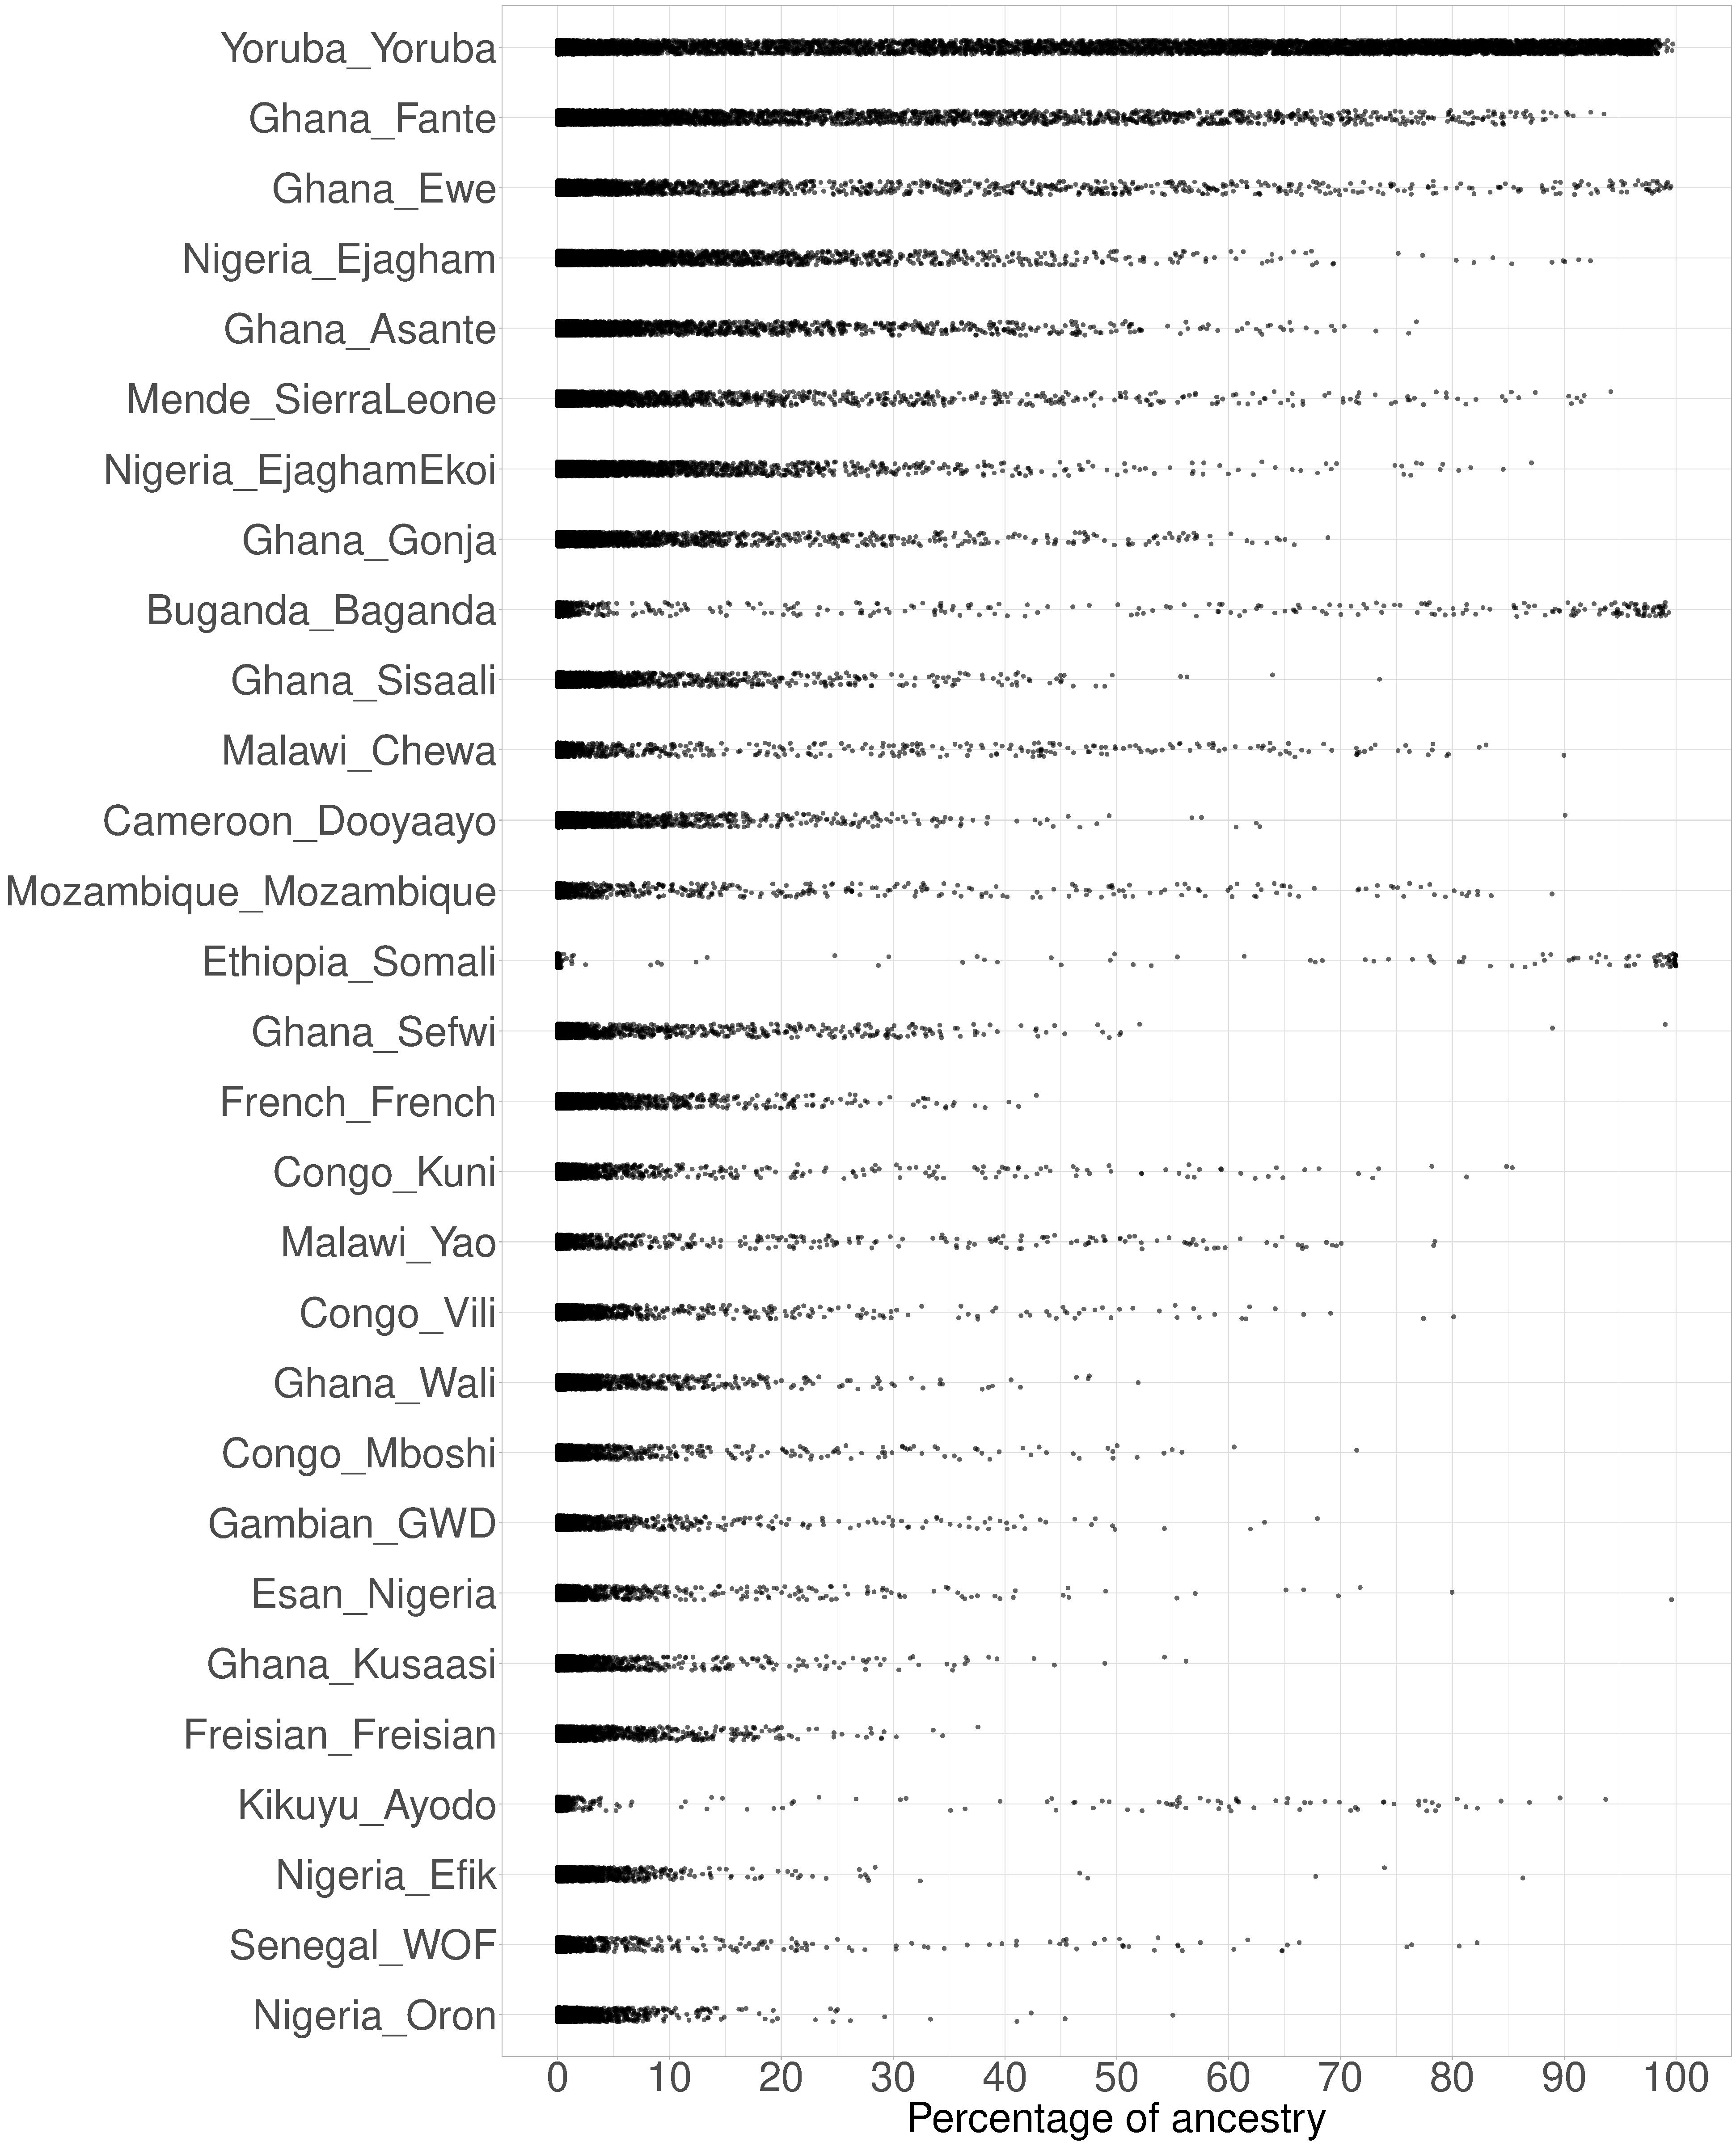
\includegraphics[width=1.0\textwidth]{../images/chapter3/SF_props_distribution_top30.pdf}
    \caption{Map of haplotype donation to UK Biobank individuals. Each point represents a different African population. Colour }
    \label{fig:SF_props_distribution_top30}
\end{figure}


\subsection{Verifying painting accuracy}

Given the total number of SNPs used in the analysis (n=65,727) is on an order of magnitude less than is typically used in such analysis, it is important to verify that the ChromoPainter results do not simply correspond to copying the most from the reference populations with the largest sample size, as has been shown in previous analyses (refer to previous chapters). To test that the coancestry matrix contains relevant information about the ancestry of the retained UK Biobank individuals, I took advantage of the UK Biobank metadata and subsetted the coancestry matrix to contain only individuals who were born in a particular country. We would expect that individuals who were born in a particular country would copy the most from reference populations from that country. For example, we would expect individuals who were born in South Africa to copy the most from Bantu and Zulu ethnic groups from South Africa. 

\begin{figure}[htp]
    \centering
    \includegraphics[width=1.0\textwidth]{../images/chapter3/haplotype_map_SouthAfrica.pdf}
    \caption{Map of haplotype donation to UK Biobank individuals born in South Africa.}
    \label{fig:haplotype_map_SouthAfrica}
\end{figure}

Fig. \ref{fig:haplotype_map_SouthAfrica} shows the map of haplotype donation from reference groups to UK Biobank individuals born in South Africa. It is clear that reference populations from South Africa, in particular the Zulu ethnic group, contribute the most to these individuals. The same pattern is clear for most countries of origin. This suggests that the painting had good resolution down to at least the level of individual countries. The pattern is qualitatively the same for all countries which had a reasonable number of donor populations. 

There are several interesting countries. For example, there are 2,263 individuals who were born in the Caribbean. Visualising the haplotype donation map for these individuals shows that they are primarily of West African ancestry, consistent with historical evidence \cite{micheletti2020genetic}. Individuals born in Brazil have ancestry from further South, again consistent with historical evidence (citation needed). However, it should be noted that there is a relatively small sample size from individuals born in Brazil (n=9), and that these individuals may not be representative of the Brazilian population. 

As a more formal test of the painting accuracy, I estimated SOURCEFIND ancestry proportions in each retained UK Biobank individual. An individual was `assigned' to a particular ethnic group if they had 75\% or more ancestry from that group. If the country the assigned reference population is from matches the birth location of the individual, then I considered that a `success' and a `fail' otherwise. Individuals who were born in the U.K. or who had no birth country were excluded from this analysis. 

\begin{figure}[htp]
    \centering
    \includegraphics[width=1.0\textwidth]{../images/chapter3/country_of_origin_allInds.pdf}
    \caption{Correspondence of true birth country with estimated birth country. Each bar corresponds to a true birth country, with the length of the bar corresponding to the total number of people in our dataset born in that country. The green section corresponds to the total number of individuals where the birth country was correctly guessed and the red section to those who were incorrectly guessed. Percentage labels give percentage correct for that country.}
    \label{fig:country_of_origin_allInds}
\end{figure}

The overall accuracy at predicting birth location was 81.63\%, suggesting there was substantial information within the coancestry matrix. For the countries where there was a large number of reference populations, such as Ghana and Nigeria, the prediction accuracy was high. For certain countries, the prediction accuracy was much lower. For example, Tanzania was only represented by a single reference population. Zimbabwe had by far the lowest prediction accuracy of the countries with more than 100 individuals at 14\%. Of the 266 individuals born in Zimbabwe, 194 were assigned to an ethnic group from outside Zimbabwe; 74 to Malawi\_Chewa, 71 to Mozambique\_Mozambique and 49 to Malawi\_Yao. Individuals from the ethnic groups from Malawi are found across Malawi, Zimbabwe and other countries, showing the possible weakness of this approach which aims to categorise individuals into a single country, as ethnic groups often transcend countries. 

I also wanted to perform the same analysis but using the data which had been imputed. This stands as a practical test of whether it is preferable to impute or retain a smaller number of non-imputed SNPs. This yielded an accuracy of 81.89\%, a value almost identical to that obtained with the dataset containing approximately 70,000 non-imputed SNPs. 


\subsection{Patterns of African ancestry across the U.K.}

The U.K. Biobank dataset also contains data on the testing centre that each individual registered at. I used this information to see whether there was structure in how different ethnicities are distributed across the U.K. There was no apparent outliers in terms of centers and the proportion of individuals who had at least 50\% African ancestry.

No clear pattern was apparent, other than Yoruba ancestry dominating most centres. 
 
I also estimated the information entropy of each centre based on the SOURCEFIND proportions. In this context, information entropy can be seen analagously to the amount of diversity in different ancestries present in a particular centre. The two centres in the two largest metropolitan areas, London and Birmingham, have the largest amount of entropy, suggesting that ethnic diversity is greater in larger cities.

\begin{sidewaysfigure}[htp]
    \centering
    \includegraphics[width=1.0\textwidth]{../images/chapter3/SF_props_pie_chart.pdf}
    \caption{Distribution of ethnicities across different testing centres. Each pie corresponds to a U.K. Biobank testing centre, with each section of the each pie corresponding to a different ethnicity.}
    \label{fig:country_of_origin_allInds}
\end{sidewaysfigure}

\section{Discussion}

In this chapter I have performed what I believe is the highest resolution analysis of African ancestry in individuals living in the U.K. I found that West African ancestry is 



